\documentclass[12pt]{article}

\usepackage{amsmath, amsthm, amssymb, amsbsy, amsfonts}
\usepackage[plainpages=false,pdfpagelabels]{hyperref}
\hypersetup{
    colorlinks,
    citecolor=black,
    filecolor=black,
    linkcolor=black,
    urlcolor=blue
}
\usepackage{verbatim}
\usepackage{enumitem}
\usepackage[utf8x]{inputenc}

% Redefine the \vec command to use bold font instead of an arrow
\renewcommand\vec[1]{\mathbf{#1}}

%\def\nl{\hfill\break\null}
\oddsidemargin=0.3cm
\topmargin=-1cm
\textwidth=15cm
\textheight=23cm
\parindent=0cm
\parskip=1mm


\usepackage{graphicx}
\DeclareMathOperator*{\argmin}{argmin}

\newenvironment{enumialpha}{\begin{enumerate}
  \def\theenumi{\alph{enumi}}
  \def\labelenumi{(\theenumi)}}{\end{enumerate}}

\newenvironment{enumiiroman}{\begin{enumerate}
  \def\theenumii{\roman{enumii}}
  \def\labelenumii{(\theenumii)}}{\end{enumerate}}


\begin{document}

\begin{tabular*}{15cm}{@{}l@{\extracolsep{\fill}}r}
  Albert-Ludwigs-Universit\"at Freiburg, Institut f\"ur Informatik \\
PD Dr. Cyrill Stachniss \\  Lecture: Robot Mapping \\
  Winter term 2013 
\end{tabular*}

\bigskip


\begin{center}
{\bf \Large Sheet 10}

{\large Topic: Graph-Based SLAM}

Submission deadline: February 3 (Task~1), February 10 (Task~2)\\
Submit to: \texttt{robotmappingtutors@informatik.uni-freiburg.de}
\end{center}

\subsubsection*{Exercise: Graph-Based SLAM}

Implement a least-squares method to address SLAM in its graph-based
formulation. To support this task, we provide a small \emph{Octave} framework (see
course website).  The framework contains the following folders:

\begin{description}
\item [data]
  contains several datasets, each gives the measurements of one SLAM
  problem
\item [octave]
  contains the Octave framework with stubs to complete.
\item [plots]
  this folder is used to store images.
\end{description}

The below mentioned tasks should be implemented inside the framework in
the directory \texttt{octave} by completing the stubs:
\begin{enumerate}
  \item
    \begin{itemize}
      \item
        Implement the function in \texttt{compute\_global\_error.m} for computing the
        current error value for a graph with constraints.
      \item
        Implement the function in
        \texttt{linearize\_pose\_pose\_constraint.m} for computing the
        error and the Jacobian of a pose-pose constraint.  Test your
        implementation with \texttt{test\_jacobian\_pose\_pose}.
      \item
        Implement the function in
        \texttt{linearize\_pose\_landmark\_constraint.m} for computing
        the error and the Jacobian of a pose-landmark constraint.  Test your
        implementation with \texttt{test\_jacobian\_pose\_landmark}.
    \end{itemize}
  \item
    \begin{itemize}
      \item
        Implement the function in \texttt{linearize\_and\_solve.m} for
        constructing and solving the linear approximation.
      \item
        Implement the update of the state vector and the stopping
        criterion in \texttt{lsSLAM.m}.  A possible choice for the
        stopping criterion is $\| \Delta \mathbf{x} \|_\infty <
        \epsilon$, i.e., $\| \Delta \mathbf{x} \|_\infty = \max \left(
        |\Delta x_1|, \ldots, |\Delta x_n| \right) < \epsilon$.
    \end{itemize}
\end{enumerate}

After implementing the missing parts, you can run the framework.  To do
that, change into the directory octave and launch \emph{Octave}. To
start the main loop, type \texttt{lsSLAM}. The script will produce a
plot showing the positions of the robot and (if available) the positions
of the landmarks in each iteration.  These plots will be saved in the
\texttt{plots} directory. 

\begin{figure}
  \centering
  {\scriptsize
  \begin{tabular}{@{}cccc@{}}
    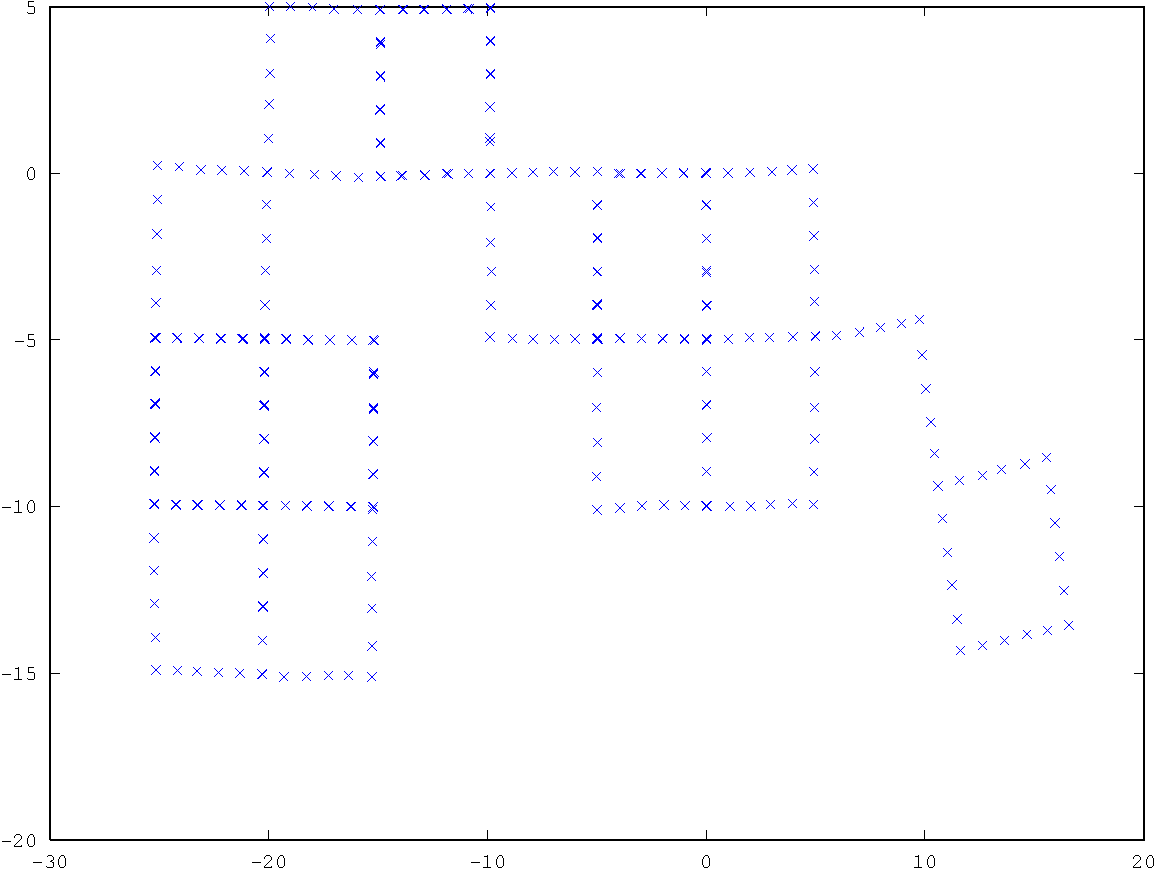
\includegraphics[width=0.22\columnwidth]{sim-pose-pose} &
    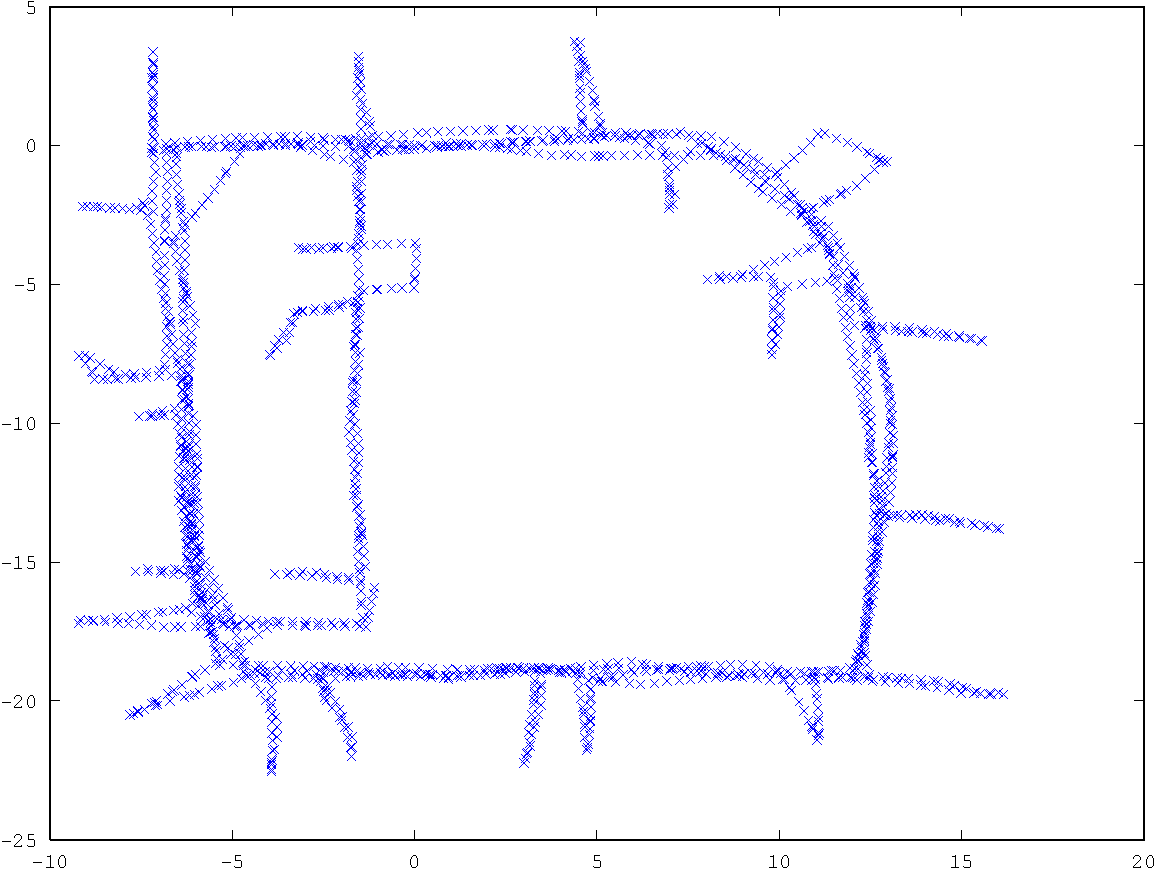
\includegraphics[width=0.22\columnwidth]{intel} &
    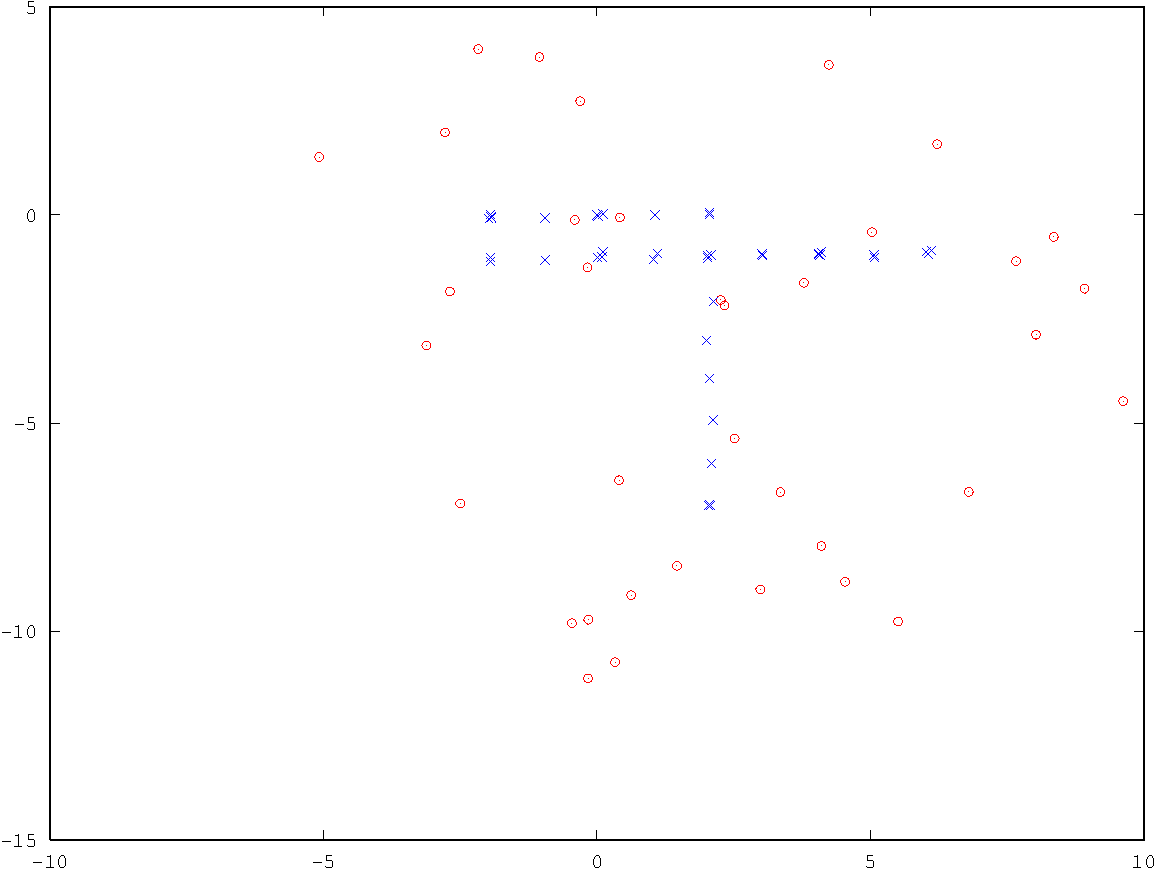
\includegraphics[width=0.22\columnwidth]{sim-pose-landmark} &
    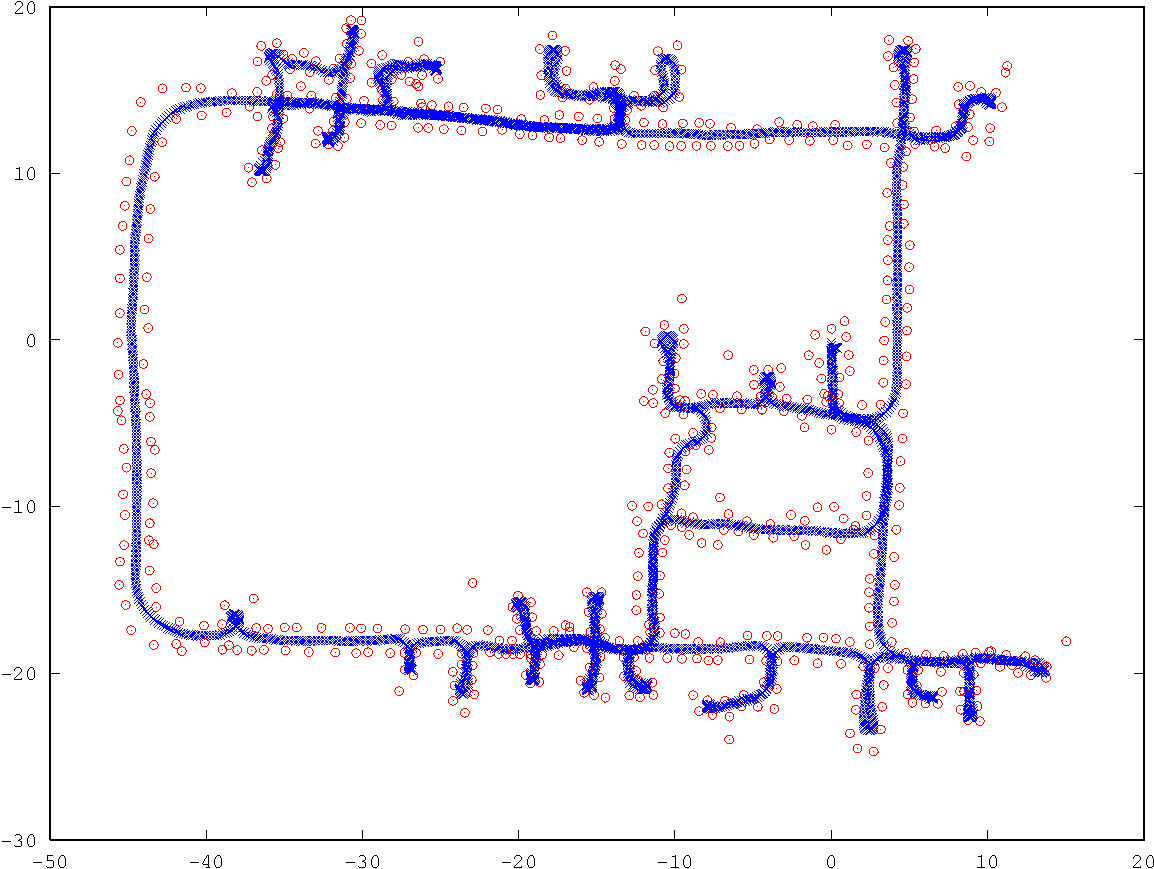
\includegraphics[width=0.22\columnwidth]{dlr}\\
    simulation-pose-pose & intel & simulation-pose-landmark & dlr
  \end{tabular}}
  \caption{Result for each dataset.}
  \label{fig:result}
\end{figure}

Figure~\ref{fig:result} depicts the result
that you should obtain after convergence for each dataset.
Additionally, the initial and the final error for each dataset should be
approximately:\\[1ex]
\begin{tabular}{|l|c|c|}
  \hline
  dataset & initial error & final error\\\hline\hline
  simulation-pose-pose.dat & 138862234 & 8269\\\hline
  intel.dat & 1795139 & 360\\\hline
  simulation-pose-landmark.dat & 3030 & 474\\\hline
  dlr.dat & 369655336 & 56860\\\hline
\end{tabular}\\

The state vector contains the following entities:
\begin{itemize}
  \item pose of the robot: $\mathbf{x}_i = (x_i \; y_i \; \theta_i)^T$\\
    Hint: You may use the function $\mathrm{v2t}(\cdot)$ and
    $\mathrm{t2v}(\cdot)$:
    \begin{align*}
    \mathrm{v2t}(\mathbf{x}_i) &= 
    \begin{pmatrix}
      R_i &\mathbf{t}_i\\
      \mathbf{0} & 1
    \end{pmatrix}
    =
    \begin{pmatrix}
      \cos(\theta_i) & -\sin(\theta_i) & x_i\\
      \sin(\theta_i) & \cos(\theta_i) & y_i\\
      0 & 0 & 1
    \end{pmatrix}
    = X_i\\
    \mathrm{t2v}(X_i) &= \mathbf{x}_i
    \end{align*}
  \item position of a landmark: $\mathbf{x}_l = (x_l \; y_l)^T$
\end{itemize}

We consider the following error functions:
\begin{itemize}
  \item pose-pose constraint:
    $\mathbf{e}_\mathit{ij} = \mathrm{t2v}(Z^{-1}_\mathit{ij} (X_i^{-1}
    X_j))$, where $Z_\mathit{ij} = \mathrm{v2t}(\mathbf{z}_\mathit{ij})$
    is the transformation matrix of the measurement $\mathbf{z}_{ij}^T =
    (\mathbf{t}_{ij}^T, \theta_{ij})$.\\
    Hint: For computing the Jacobian, write the error function with
    rotation matrices and translation vectors:
    \begin{align*}
      \mathbf{e}_\mathit{ij} &=
      \begin{pmatrix}
        R_{ij}^T (R_i^T(\mathbf{t}_j-\mathbf{t}_i)-\mathbf{t}_{ij})\\
        \theta_j -\theta_i - \theta_{ij}\\
      \end{pmatrix}
    \end{align*}
  \item pose-landmark constraint:
    $\mathbf{e}_\mathit{il} = R_i^T (\mathbf{x}_l - \mathbf{t}_i) -
    \mathbf{z}_{il}$
\end{itemize}

%Some implementation tips:
%\begin{itemize}
%\item
  %The functions v2t($\cdot$) and t2v($\cdot$) to convert
  %between a pose vector and a transformation matrix are available in the
  %Octave framework.
%\item
  %You may first implement the functions in
  %\texttt{linearize\_pose\_pose\_constraint.m} and apply the framework
  %to the datasets which do not contain landmarks.
%\item
  %When solving the linear system exploit the sparseness of the matrix.
  %You may resort to the backslash operator.
%\item
  %Many of the functions in \emph{Octave} can handle matrices and
  %compute values along the rows or columns of a matrix. Some useful
  %functions that support this are \texttt{max}, \texttt{abs}, \texttt{sum},  \texttt{log},
  %\texttt{sqrt}, \texttt{sin}, \texttt{cos}, and many others.
%\end{itemize}

\end{document}
